	%%%%%%%% ICML 2018 EXAMPLE LATEX SUBMISSION FILE %%%%%%%%%%%%%%%%%

\documentclass{article}
\usepackage{icml2018}

\usepackage[utf8]{inputenc} % allow utf-8 input
\usepackage[T1]{fontenc}    % use 8-bit T1 fonts
\usepackage{url}            % simple URL typesetting
\usepackage{booktabs}       % professional-quality tables
\usepackage{amsfonts}       % blackboard math symbols
\usepackage{nicefrac}       % compact symbols for 1/2, etc.
\usepackage{microtype}      % microtypography
\usepackage{times}
\usepackage{mathtools}
% Packages hyperref and algorithmic misbehave sometimes.  We can fix
% this with the following command.
%\newcommand{\theHalgorithm}{\arabic{algorithm}}
\usepackage{graphicx} % more modern
%\usepackage{epsfig} % less modern
%\usepackage{subfigure} 
\usepackage{subcaption}

% For citations

% For algorithms
\usepackage{algorithm}
\usepackage{algorithmic}
\usepackage{multirow}
\usepackage{amsthm}
\usepackage{mathrsfs}
\usepackage{graphicx}
\usepackage{caption}%, subcaption}
\usepackage{xspace}
\usepackage{float}
\usepackage{wrapfig}
\usepackage{enumitem}
\usepackage{wrapfig}
\setitemize{noitemsep,topsep=0pt,parsep=2pt,partopsep=0pt}
\usepackage{natbib}
\usepackage{caption}
\usepackage{multibib} % hack to have appendix cites separately
% after compiling as usual, you also need to additionally run
%      bibtex sup
% once to get the second bibliography in the appendix
\newcites{sup}{Supplementary References}
\usepackage{hyperref}       % hyperlinks
\usepackage[font = footnotesize]{caption}
%% to get the right citation format
%\renewcommand{\citesup}{\cite}

% Use the following line for the initial blind version submitted for review:
\def\R{{\mathbb{R}}}

%-------------
\def\etal{et\/ al.\/ }
\def\bydef{:=}
\def\th{{^{th}}}
\def\suchthat{\text{s.t.}}

% %-------------
\def\embed{\hookrightarrow}
\def\to{{\,\rightarrow\,}}
\def\kron{\otimes}
\def\had{\circ}
\def\ksum{\oplus}

\mathchardef\mhyphen="2D
\newcommand{\smallmat}[1]{\left[\begin{smallmatrix}#1\end{smallmatrix}\right]}
\newcommand{\smallmt}[1]{\begin{smallmatrix}#1\end{smallmatrix}}


%-------------
%\let\vec\vec
\newcommand{\tvec}[1]{{\text{vec}(#1)}}
\newcommand{\mat}[1]{{\text{mat}(#1)}} %omega subindex
\newcommand{\indicator}[1]{ {\mathsf{1}}_{\left[ {#1} \right] }}

\def\half{\frac{1}{2}}
\newcommand{\fracl}[1]{\frac{1}{#1}}
\providecommand{\abs}[1]{{\left\lvert#1\right\rvert}}
\providecommand{\trans}[1]{{#1^\top}}
\providecommand{\inv}[1]{{#1^{-1}}}
\providecommand{\inner}[2]{{\left\langle#1, #2\right\rangle}}
\providecommand{\innere}[2]{{\trans{#1}#2}}
\providecommand{\innerd}[2]{{#1{\boldsymbol{\cdot}}#2}}
\providecommand{\brac}[1]{{\left(#1\right)}}

\providecommand{\dot}[2]{{\trans{#1}#2}}
\newcommand{\tr}[1]{{\mathrm{tr}}\!\left( #1 \right)}
\newcommand{\kl}[2]{{\mathrm{KL}\!\left({#1}\Vert{#2}\right)}}
\newcommand{\Hp}[1]{{\mathrm{H}\!\left({#1}\right)}}
\newcommand{\Hpp}[1]{-\Hp{#1}}

% vector norms:
\newcommand{\norm}[1]{{ \left\lVert#1\right\rVert }}
\newcommand{\normb}[1]{\norm{#1}_2}
\newcommand{\normbs}[1]{\normb{#1}^2}

% matrix norm
\newcommand{\vertiii}[1]{{\left\vert\kern-0.25ex\left\vert\kern-0.25ex\left\vert #1
    \right\vert\kern-0.25ex\right\vert\kern-0.25ex\right\vert}}

\newcommand{\normf}[1]{\vertiii{#1}_2}
\newcommand{\normfs}[1]{\normf{#1}^2}
\newcommand{\normt}[1]{\vertiii{#1}_1}
\newcommand{\normr}[1]{\vertiii{#1}_0}

\newcommand{\normh}[2]{\vertiii{#1}_{2 \mhyphen #2}}
\newcommand{\normhs}[2]{\normh{#1}{#2}^2}
\newcommand{\normht}[2]{\vertiii{#1}_{1 \mhyphen #2}}
\newcommand{\normhr}[2]{\vertiii{#1}_{0\,\mhyphen #2}}

\newcommand{\gp}[2]{\cG\cP \left(#1, #2\right)}
\newcommand{\gpv}[3]{\cM\cG\cP \left(#1, #2, #3\right)}
\newcommand{\g}[2]{\cN\left(#1, #2\right)}
\newcommand{\gv}[3]{\cM\cN \left(#1, #2, #3\right)}
\newcommand{\etr}[1]{\text{etr}\left( #1 \right)}
%\newcommand{\ev}[2]{\mathrm{E}_{ #1}\left[ #2 \right]}
%\newcommand{\ev}[2]{\mathrm{E}_{ #1}\left[ \, #2 \, \right]}
%\newcommand{\evb}[2]{\ev{}{#2}\left(#1\right)}
\newcommand{\expf}[1]{ \exp \left( #1 \right) }
\newcommand{\exf}[1]{ e^{ #1 } }
\def\sut{\text{s.t.}}


%-------------Gradients
\newcommand{\D}[2]{\frac{d #1}{d #2}} % for derivatives
\newcommand{\dd}[2]{\frac{d^2 #1}{d #2^2}} % for double derivatives
\newcommand{\pd}[2]{\frac{\partial #1}{\partial #2}}
\newcommand{\pdd}[2]{\frac{\partial^2 #1}{\partial #2^2}}
\newcommand{\gradb}[1]{\gv{\nabla} #1}
\newcommand{\grad}[1]{ \nabla_{#1} }

\newcommand{\vect}[1]{{\boldsymbol{#1}}}

\newcommand{\EE}[1]{ \mathbb{E}\left[#1\right] }
%-------------
\def\eps{\epsilon}
% bold greek symbols
\def\balpha{\vect{\alpha}}
\def\bbeta{\vect{\beta}}
\def\bmu{\vect{\mu}}
\def\bnu{\vect{\nu}}
\def\beps{\vect{\epsilon}}
\def\bphi{\vect{\phi}}
\def\bpsi{\vect{\psi}}
\def\btheta{\vect{\theta}}
\def\bpi{\vect{\pi}}
\def\bgamma{\vect{\gamma}}
\def\beeta{\vect{\eta}}
\def\blambda{\vect{\lambda}}
\def\bkappa{\vect{\kappa}}
\def\bupsilon{\vect{\upsilon}}
\def\bomega{\vect{\omega}}
\def\btau{\vect{\tau}}
\def\brho{\vect{\rho}}
\def\bchi{\vect{\chi}}
%------------- capitals
\def\bPi{\vect{\Pi}}
\def\bPsi{\vect{\Psi}}
\def\bPhi{\vect{\Phi}}
\def\bTheta{\vect{\Theta}}
\def\bSigma{\vect{\Sigma}}
\def\bLambda{\vect{\Lambda}}
\def\bOmega{\vect{\Omega}}
\def\bDelta{\vect{\Delta}}
\def\bUpsilon{\vect{\Upsilon}}
\def\bAlpha{\vect{\vA}}
\def\bGamma{\vect{\Gamma}}
\def\bAlpha{\vect{A}}

% vect lowercase
\def\va{{\vect{a}}}
\def\vb{{\vect{b}}}
\def\vc{{\vect{c}}}
\def\vd{{\vect{d}}}
\def\vee{{\vect{e}}}
\def\vff{{\vect{f}}}
\def\vg{{\vect{g}}}
\def\vh{{\vect{h}}}
\def\vi{{\vect{i}}}
\def\vk{{\vect{k}}}
\def\vl{{\vect{l}}}
\def\vm{{\vect{m}}}
\def\vn{{\vect{n}}}
\def\vo{{\vect{o}}}
\def\vp{{\vect{p}}}
\def\vq{{\vect{q}}}
\def\vr{{\vect{r}}}
\def\vs{{\vect{s}}}
\def\vt{{\vect{t}}}
\def\vu{{\vect{u}}}
\def\vv{{\vect{v}}}
\def\vw{{\vect{w}}}
\def\vx{{\vect{x}}}
\def\vy{{\vect{y}}}
\def\vz{{\vect{z}}}
%-------------
% vect capital letters
\def\vA{{\vect{A}}}
\def\vB{{\vect{B}}}
\def\vC{{\vect{C}}}
\def\vD{{\vect{D}}}
\def\vE{{\vect{E}}}
\def\vF{{\vect{F}}}
\def\vG{{\vect{G}}}
\def\vH{{\vect{H}}}
\def\vI{{\vect{I}}}
\def\vJ{{\vect{J}}}
\def\vK{{\vect{K}}}
\def\vL{{\vect{L}}}
\def\vM{{\vect{M}}}
\def\vN{{\vect{N}}}
\def\vO{{\vect{O}}}
\def\vP{{\vect{P}}}
\def\vQ{{\vect{Q}}}
\def\vR{{\vect{R}}}
\def\vS{{\vect{S}}}
\def\vT{{\vect{T}}}
\def\vU{{\vect{U}}}
\def\vV{{\vect{V}}}
\def\vW{{\vect{W}}}
\def\vX{{\vect{X}}}
\def\vY{{\vect{Y}}}
\def\vZ{{\vect{Z}}}

%-------------
% Bold lowercase
\def\ba{{\mathbf{a}}}
\def\bb{{\mathbf{b}}}
\def\bc{{\mathbf{c}}}
\def\bd{{\mathbf{d}}}
\def\be{{\mathbf{e}}}
\def\bff{{\mathbf{f}}}
\def\bg{{\mathbf{g}}}
\def\bh{{\mathbf{h}}}
\def\bi{{\mathbf{i}}}
\def\bj{{\mathbf{j}}}
\def\bk{{\mathbf{k}}}
\def\bl{{\mathbf{l}}}
\def\bm{{\mathbf{m}}}
\def\bn{{\mathbf{n}}}
\def\bo{{\mathbf{o}}}
\def\bp{{\mathbf{p}}}
\def\bq{{\mathbf{q}}}
\def\br{{\mathbf{r}}}
\def\bs{{\mathbf{s}}}
\def\bt{{\mathbf{t}}}
\def\bu{{\mathbf{u}}}
\def\bv{{\mathbf{v}}}
\def\bw{{\mathbf{w}}}
\def\bx{{\mathbf{x}}}
\def\by{{\mathbf{y}}}
\def\bz{{\mathbf{z}}}
%-------------
% Bold capital letters
\def\bA{{\mathbf{A}}}
\def\bB{{\mathbf{B}}}
\def\bC{{\mathbf{C}}}
\def\bD{{\mathbf{D}}}
\def\bE{{\mathbf{E}}}
\def\bF{{\mathbf{F}}}
\def\bG{{\mathbf{G}}}
\def\bH{{\mathbf{H}}}
\def\bI{{\mathbf{I}}}
\def\bJ{{\mathbf{J}}}
\def\bK{{\mathbf{K}}}
\def\bL{{\mathbf{L}}}
\def\bM{{\mathbf{M}}}
\def\bN{{\mathbf{N}}}
\def\bO{{\mathbf{O}}}
\def\bP{{\mathbf{P}}}
\def\bQ{{\mathbf{Q}}}
\def\bR{{\mathbf{R}}}
\def\bS{{\mathbf{S}}}
\def\bT{{\mathbf{T}}}
\def\bU{{\mathbf{U}}}
\def\bV{{\mathbf{V}}}
\def\bW{{\mathbf{W}}}
\def\bX{{\mathbf{X}}}
\def\bY{{\mathbf{Y}}}
\def\bZ{{\mathbf{Z}}}

\def\0{{\mathbf{0}}}

%-------------
% bold arrow-vect lowercase
\def\aa{{\vec{\ba}}}
\def\ab{{\vec{\bb}}}
\def\ac{{\vec{\bc}}}
\def\ad{{\vec{\bd}}}
\def\aee{{\vec{\be}}}
\def\aff{{\vec{\bf}}}
\def\ag{{\vec{\bg}}}
\def\ah{{\vec{\bh}}}
\def\ai{{\vec{\bi}}}
\def\ak{{\vec{\bk}}}
\def\al{{\vec{\bl}}}
\def\am{{\vec{\bm}}}
\def\an{{\vec{\bn}}}
\def\ao{{\vec{\bo}}}
\def\ap{{\vec{\bp}}}
\def\aq{{\vec{\bq}}}
\def\ar{{\vec{\br}}}
\def\as{{\vec{\bs}}}
\def\at{{\vec{\bt}}}
\def\au{{\vec{\bu}}}
\def\av{{\vec{\bv}}}
\def\aw{{\vec{\bw}}}
\def\ax{{\vec{\bx}}}
\def\ay{{\vec{\by}}}
\def\az{{\vec{\bz}}}
%-------------
% bold arrow-vect capital letters
\def\aA{{\vec{\bA}}}
\def\aB{{\vec{\bB}}}
\def\aC{{\vec{\bC}}}
\def\aD{{\vec{\bD}}}
\def\aE{{\vec{\bE}}}
\def\aF{{\vec{\bF}}}
\def\aG{{\vec{\bG}}}
\def\aH{{\vec{\bH}}}
\def\aI{{\vec{\bI}}}
\def\aJ{{\vec{\bJ}}}
\def\aK{{\vec{\bK}}}
\def\aL{{\vec{\bL}}}
\def\aM{{\vec{\bM}}}
\def\aN{{\vec{\bN}}}
\def\aO{{\vec{\bO}}}
\def\aP{{\vec{\bP}}}
\def\aQ{{\vec{\bQ}}}
\def\aR{{\vec{\bR}}}
\def\aS{{\vec{\bS}}}
\def\aT{{\vec{\bT}}}
\def\aU{{\vec{\bU}}}
\def\aV{{\vec{\bV}}}
\def\aW{{\vec{\bW}}}
\def\aX{{\vec{\bX}}}
\def\aY{{\vec{\bY}}}
\def\aZ{{\vec{\bZ}}}

%-------------
% blackboard lowercase
\def\bba{{\mathbb{a}}}
\def\bbb{{\mathbb{b}}}
\def\bbc{{\mathbb{c}}}
\def\bbd{{\mathbb{d}}}
\def\bbee{{\mathbb{e}}}
\def\bbff{{\mathbb{f}}}
\def\bbg{{\mathbb{g}}}
\def\bbh{{\mathbb{h}}}
\def\bbi{{\mathbb{i}}}
\def\bbj{{\mathbb{j}}}
\def\bbk{{\mathbb{k}}}
\def\bbl{{\mathbb{l}}}
\def\bbm{{\mathbb{m}}}
\def\bbn{{\mathbb{n}}}
\def\bbo{{\mathbb{o}}}
\def\bbp{{\mathbb{p}}}
\def\bbq{{\mathbb{q}}}
\def\bbr{{\mathbb{r}}}
\def\bbs{{\mathbb{s}}}
\def\bbt{{\mathbb{t}}}
\def\bbu{{\mathbb{u}}}
\def\bbv{{\mathbb{v}}}
\def\bbw{{\mathbb{w}}}
\def\bbx{{\mathbb{x}}}
\def\bby{{\mathbb{y}}}
\def\bbz{{\mathbb{z}}}
%-------------
% Blackboard capital letters
\def\bbA{{\mathbb{A}}}
\def\bbB{{\mathbb{B}}}
\def\bbC{{\mathbb{C}}}
\def\bbD{{\mathbb{D}}}
\def\bbE{{\mathbb{E}}}
\def\bbF{{\mathbb{F}}}
\def\bbG{{\mathbb{G}}}
\def\bbH{{\mathbb{H}}}
\def\bbI{{\mathbb{I}}}
\def\bbJ{{\mathbb{J}}}
\def\bbK{{\mathbb{K}}}
\def\bbL{{\mathbb{L}}}
\def\bbM{{\mathbb{M}}}
\def\bbN{{\mathbb{N}}}
\def\bbO{{\mathbb{O}}}
\def\bbP{{\mathbb{P}}}
\def\bbQ{{\mathbb{Q}}}
\def\bbR{{\mathbb{R}}}
\def\bbS{{\mathbb{S}}}
\def\bbT{{\mathbb{T}}}
\def\bbU{{\mathbb{U}}}
\def\bbV{{\mathbb{V}}}
\def\bbW{{\mathbb{W}}}
\def\bbX{{\mathbb{X}}}
\def\bbY{{\mathbb{Y}}}
\def\bbZ{{\mathbb{Z}}}
%-------------
% Caligraphic capital letters
\def\cA{\mathcal{A}}
\def\cB{\mathcal{B}}
\def\cC{\mathcal{C}}
\def\cD{\mathcal{D}}
\def\cE{\mathcal{E}}
\def\cF{\mathcal{F}}
\def\cG{\mathcal{G}}
\def\cH{\mathcal{H}}
\def\cI{\mathcal{I}}
\def\cJ{\mathcal{J}}
\def\cK{\mathcal{K}}
\def\cL{\mathcal{L}}
\def\cM{\mathcal{M}}
\def\cN{\mathcal{N}}
\def\cO{\mathcal{O}}
\def\cP{\mathcal{P}}
\def\cQ{\mathcal{Q}}
\def\cR{\mathcal{R}}
\def\cS{\mathcal{S}}
\def\cT{\mathcal{T}}
\def\cU{\mathcal{U}}
\def\cV{\mathcal{V}}
\def\cW{\mathcal{W}}
\def\cX{\mathcal{X}}
\def\cY{\mathcal{Y}}
\def\cZ{\mathcal{Z}}
%-------------
% sans serif lowercase
\def\sfa{{\mathsf{a}}}
\def\sfb{{\mathsf{b}}}
\def\sfc{{\mathsf{c}}}
\def\sfd{{\mathsf{d}}}
\def\sfee{{\mathsf{e}}}
\def\sfff{{\mathsf{f}}}
\def\sfg{{\mathsf{g}}}
\def\sfh{{\mathsf{h}}}
\def\sfi{{\mathsf{i}}}
\def\sfj{{\mathsf{j}}}
\def\sfk{{\mathsf{k}}}
\def\sfl{{\mathsf{l}}}
\def\sfm{{\mathsf{m}}}
\def\sfn{{\mathsf{n}}}
\def\sfo{{\mathsf{o}}}
\def\sfp{{\mathsf{p}}}
\def\sfq{{\mathsf{q}}}
\def\sfr{{\mathsf{r}}}
\def\sfs{{\mathsf{s}}}
\def\sft{{\mathsf{t}}}
\def\sfu{{\mathsf{u}}}
\def\sfv{{\mathsf{v}}}
\def\sfw{{\mathsf{w}}}
\def\sfx{{\mathsf{x}}}
\def\sfy{{\mathsf{y}}}
\def\sfz{{\mathsf{z}}}
%-------------
% Sans serif capital letters
\def\sfA{\mathsf{A}}
\def\sfB{\mathsf{B}}
\def\sfC{\mathsf{C}}
\def\sfD{\mathsf{D}}
\def\sfE{\mathsf{E}}
\def\sfF{\mathsf{F}}
\def\sfG{\mathsf{G}}
\def\sfH{\mathsf{H}}
\def\sfI{\mathsf{I}}
\def\sfJ{\mathsf{J}}
\def\sfK{\mathsf{K}}
\def\sfL{\mathsf{L}}
\def\sfM{\mathsf{M}}
\def\sfN{\mathsf{N}}
\def\sfO{\mathsf{O}}
\def\sfP{\mathsf{P}}
\def\sfQ{\mathsf{Q}}
\def\sfR{\mathsf{R}}
\def\sfS{\mathsf{S}}
\def\sfT{\mathsf{T}}
\def\sfU{\mathsf{U}}
\def\sfV{\mathsf{V}}
\def\sfW{\mathsf{W}}
\def\sfX{\mathsf{X}}
\def\sfY{\mathsf{Y}}
\def\sfZ{\mathsf{Z}}
%-------------
% frak lowercase
\def\fra{{\mathfrak{a}}}
\def\frb{{\mathfrak{b}}}
\def\frc{{\mathfrak{c}}}
\def\frd{{\mathfrak{d}}}
\def\free{{\mathfrak{e}}}
\def\frff{{\mathfrak{f}}}
\def\frg{{\mathfrak{g}}}
\def\frh{{\mathfrak{h}}}
\def\fri{{\mathfrak{i}}}
\def\frj{{\mathfrak{j}}}
\def\frk{{\mathfrak{k}}}
\def\frl{{\mathfrak{l}}}
\def\frm{{\mathfrak{m}}}
\def\frn{{\mathfrak{n}}}
\def\fro{{\mathfrak{o}}}
\def\frp{{\mathfrak{p}}}
\def\frq{{\mathfrak{q}}}
\def\frr{{\mathfrak{r}}}
\def\frs{{\mathfrak{s}}}
\def\frt{{\mathfrak{t}}}
\def\fru{{\mathfrak{u}}}
\def\frv{{\mathfrak{v}}}
\def\frw{{\mathfrak{w}}}
\def\frx{{\mathfrak{x}}}
\def\fry{{\mathfrak{y}}}
\def\frz{{\mathfrak{z}}}
%-------------
% frak Capital letters
\def\frA{\mathfrak{A}}
\def\frB{\mathfrak{B}}
\def\frC{\mathfrak{C}}
\def\frD{\mathfrak{D}}
\def\frE{\mathfrak{E}}
\def\frF{\mathfrak{F}}
\def\frG{\mathfrak{G}}
\def\frH{\mathfrak{H}}
\def\frI{\mathfrak{I}}
\def\frJ{\mathfrak{J}}
\def\frK{\mathfrak{K}}
\def\frL{\mathfrak{L}}
\def\frM{\mathfrak{M}}
\def\frN{\mathfrak{N}}
\def\frO{\mathfrak{O}}
\def\frP{\mathfrak{P}}
\def\frQ{\mathfrak{Q}}
\def\frR{\mathfrak{R}}
\def\frS{\mathfrak{S}}
\def\frT{\mathfrak{T}}
\def\frU{\mathfrak{U}}
\def\frV{\mathfrak{V}}
\def\frW{\mathfrak{W}}
\def\frX{\mathfrak{X}}
\def\frY{\mathfrak{Y}}
\def\frZ{\mathfrak{Z}}


%repeating theorems
\newtheorem*{rep@theorem}{\rep@title}
\newcommand{\newreptheorem}[2]{%
\newenvironment{rep#1}[1]{%
 \def\rep@title{#2 \ref{##1}}%
 \begin{rep@theorem}}%
 {\end{rep@theorem}}}
\newreptheorem{lemma}{Lemma'}
\newreptheorem{definition}{Definition'}
\newreptheorem{proposition}{Proposition'}
\newreptheorem{theorem}{Theorem'}

%%--------------
\newtheorem{theorem}{Theorem}
%\newtheorem{acknowledgement}[theorem]{Acknowledgement}
%\newtheorem{assumption}[theorem]{Assumption}
\newtheorem{definition}[theorem]{Definition}
%\newtheorem{algorithm}[theorem]{Algorithm}
%\newtheorem{axiom}[theorem]{Axiom}
%\newtheorem{case}[theorem]{Case}
%\newtheorem{claim}[theorem]{Claim}
%\newtheorem{conclusion}[theorem]{Conclusion}
\newtheorem{condition}[theorem]{Condition}
%\newtheorem{conjecture}[theorem]{Conjecture}
\newtheorem{corollary}[theorem]{Corollary}
%\newtheorem{criterion}[theorem]{Criterion}
%\newtheorem{definition}[theorem]{Definition}
%\newtheorem{example}[theorem]{Example}
%\newtheorem{exercise}[theorem]{Exercise}
%\newtheorem{fact}[theorem]{Fact}
\newtheorem{lemma}[theorem]{Lemma}
%%\newtheorem{notation}[theorem]{Notation}
%\newtheorem{problem}[theorem]{Problem}
\newtheorem{proposition}[theorem]{Proposition}
%\newtheorem{solution}[theorem]{Solution}
%\newtheorem{summary}[theorem]{Summary}
%%\newtheorem{remark}[theorem]{Remark}
%\newtheorem{corollary}{Corollary}
%\newtheorem{remark}{Remark}
%-------------
%\renewcommand{\text}[1]{{\mathrm{#1}}}
\renewcommand{\text}[1]{{\textnormal{#1}}}

%%--------------
\newcommand{\figref}[1]{{Fig.}~\ref{#1}}
\newcommand{\secref}[1]{{Section}~\ref{#1}}
\newcommand{\Secref}[1]{{Section}~\ref{#1}}
\newcommand{\tabref}[1]{{Table}~\ref{#1}}
\newcommand{\thref}[1]{{Theorem}~\ref{#1}}
%\newcommand{\algref}[1]{{Algorithm}~\ref{#1}}
\newcommand{\aref}[1]{{Algorithm}~\ref{#1}}
\newcommand{\propref}[1]{{Proposition}~\ref{#1}}
\newcommand{\lemref}[1]{{Lemma}~\ref{#1}}
\newcommand{\corref}[1]{{Corollary}~\ref{#1}}
\newcommand{\chref}[1]{{Chapter}~\ref{#1}}
\newcommand{\defref}[1]{{Definiton}~\ref{#1}}

\usepackage{xcolor}
\newcommand{\FL}[1]{\textbf{\color{violet}FL:}{~\color{cyan}#1}}
\newcommand{\DV}[1]{\textbf{\color{red}DV:}{~\color{red}#1}}
\usepackage{footnote}
\makesavenoteenv{tabular}
\newcommand{\Pd}{P_{d}}
\newcommand{\Pm}{P_{model}}
\DeclareMathOperator*{\argmin}{arg\,min}
\DeclareMathOperator*{\argmax}{arg\,max}
% If accepted, instead use the following line for the camera-ready submission:
%\usepackage[accepted]{icml2018}

% The \icmltitle you define below is probably too long as a header.
% Therefore, a short form for the running title is supplied here:
\icmltitlerunning{kVAEs: Training Mixtures of VAEs}

\begin{document}

\twocolumn[
\icmltitle{Clustering Meets Implicit Generative Models: A Case For VAEs}

% It is OKAY to include author information, even for blind
% submissions: the style file will automatically remove it for you
% unless you've provided the [accepted] option to the icml2018
% package.

% List of affiliations: The first argument should be a (short)
% identifier you will use later to specify author affiliations
% Academic affiliations should list Department, University, City, Region, Country
% Industry affiliations should list Company, City, Region, Country

% You can specify symbols, otherwise they are numbered in order.
% Ideally, you should not use this facility. Affiliations will be numbered
% in order of appearance and this is the preferred way.
\icmlsetsymbol{equal}{*}

\begin{icmlauthorlist}
\icmlauthor{Aeiau Zzzz}{equal,to}
\icmlauthor{Bauiu C.~Yyyy}{equal,to,goo}
\icmlauthor{Cieua Vvvvv}{goo}
\icmlauthor{Iaesut Saoeu}{ed}
\icmlauthor{Fiuea Rrrr}{to}
\icmlauthor{Tateu H.~Yasehe}{ed,to,goo}
\icmlauthor{Aaoeu Iasoh}{goo}
\icmlauthor{Buiui Eueu}{ed}
\icmlauthor{Aeuia Zzzz}{ed}
\icmlauthor{Bieea C.~Yyyy}{to,goo}
\icmlauthor{Teoau Xxxx}{ed}
\icmlauthor{Eee Pppp}{ed}
\end{icmlauthorlist}

\icmlaffiliation{to}{Department of Computation, University of Torontoland, Torontoland, Canada}
\icmlaffiliation{goo}{Googol ShallowMind, New London, Michigan, USA}
\icmlaffiliation{ed}{School of Computation, University of Edenborrow, Edenborrow, United Kingdom}

\icmlcorrespondingauthor{Cieua Vvvvv}{c.vvvvv@googol.com}
\icmlcorrespondingauthor{Eee Pppp}{ep@eden.co.uk}

% You may provide any keywords that you
% find helpful for describing your paper; these are used to populate
% the "keywords" metadata in the PDF but will not be shown in the document
\icmlkeywords{Machine Learning, ICML}

\vskip 0.3in
]

% this must go after the closing bracket ] following \twocolumn[ ...

% This command actually creates the footnote in the first column
% listing the affiliations and the copyright notice.
% The command takes one argument, which is text to display at the start of the footnote.
% The \icmlEqualContribution command is standard text for equal contribution.
% Remove it (just {}) if you do not need this facility.

%\printAffiliationsAndNotice{}  % leave blank if no need to mention equal contribution
\printAffiliationsAndNotice{\icmlEqualContribution} % otherwise use the standard text.

\begin{abstract}
TODO
\end{abstract}

\section{Introduction}
In recent years, generative models have attracted significant attention which resulted in many success stories in machine learning. Generative models are trained from unlabelled data and are capable of generating samples which resemble the ones from the training distribution. This task is of crucial importance for the machine learning community as it is a fundamental component of unsupervised learning.
Two of the most prominent representative are Generative Adversarial Networks (GANs)~\cite{goodfellow2014generative} and Variational Autoencoders~\cite{kingma2013auto}. Both approaches aim at minimizing the discrepancy between the true data distribution and the one learned by the model. The model distribution is typically parametrized with a neural network which transforms random vectors into samples in the space of the training data (for example a picture space). Variational Autencoders are based on an elegant bayesian interpretation. They maximize the log likelihood and are able to perform efficient approximate inference on probabilistic models with continuous latent variables and intractable posterior. Furthermore, they come with an encoder network which maps data points to the latent space. On the other hand, VAEs are known to produce blurry samples when applied to natural images. GANs take a completely different approach, relying on adversarial training. This resulted in impressive empirically results. On the contrary, GANs are notoriously hard to train and suffer from the \textit{mode collapse} problem. Indeed, if the data distribution lays outside the class of functions that the generator network can learn the latter will ignore portions of the former and focus on the parts which can be approximated well given its limited capacity. An enormous effort have been made by the community to tackle this problem and several different approaches were proposed. The most relevant to our setting is the work of~\cite{Tolstikhin:2017wo} who proposed to train multiple generators, one after the others. As long as each generator collapse on a different mode, and given a large enough number of generators, one can approximate the whole data distribution by combining them. Several works followed up, trying to avoid the sequential training of the generator, most notably \cite{hoang2017multi} proposed to train multiple generators in parallel using adversarial training and a classifier to help them separate to different modes.
Instead, Variational Autoencoders stands at the other extreme suffering infinite loss if they do not model the whole support of the data distribution. We aim at bridging this gap developing a general approach to train multiple generators in parallel which focus on different parts of the training distribution. We particularize this framework for VAEs. As a consequence, each VAE will be able to collapse on some mode while the mixture of generators (decoders) will still approximate the data distribution.

Borrowing ideas from both the clustering and the causality literature we assume that the data was generated by \textit{independent mechanisms}. This assumption states that the each random variable in the system is independent from the others given its parents. In other words, the generative process is composed of separate modules that do not inform nor interfere with each other. Furthermore, any knowledge of one of these modules do not bring any knowledge about the others. In this setting, each training point was generated by an unknown mechanism and we get to observe only a mixture of these realizations. Recovering the mechanism is a hard and ill posed inverse problem. A critical assumption is that the true causal conditional distribution is the simplest among all the possible factorizations of the random variables. Simplicity can be measured with the \textit{Kolmogorov Complexity}~\cite{janzing2010causal}. 
Inspired by these notions, we aim at approximating the data distribution by dividing it in different components with non overlapping support. Then, each  part can be approximated by an independent generative model. In this way, we allow VAEs to learn only a fraction of the data distribution. As a consequence, they are able to model each part of the distribution better than a single model trying to approximate the whole data distribution. While the optimal split of the data distribution is unknown, we rely on a competitive procedure based on a set of discriminators to separate the data into the different mechanisms. Each training point will be won by the model which generates the most similar samples according to the discriminators.  Intuitively, a model that approximates the true causal mechanism will be easier to learn. Therefore, we exploit the implicit regularization given by the parametric form the networks to split the data in a way which is simple for them to learn.

In this paper we design a training procedure to split the data distribution into components which are approximated by independent generative models. This approach has several benefits:
\begin{itemize}
\item We provide a clear algorithmic framework for training mixtures of generative models. We target the most abstract case of minimizing a general $f$-divergence using a mixture of generators. Furthermore, we show convergence of the training procedure to the minimizer of the empirical estimate of the divergence
\item We particularize our framework to mixtures of VAEs. By doing so, we allow them to collapse on separate modes of the distribution. As a consequence, we force the VAEs to produce the samples strictly inside the support of the data distribution.
\item We present a clustering interpretation of our approach in non metric spaces and recover  k-means as a special case.
\item We provide empirical evidence that shows that the training procedure do split the training distribution into semantically different components which also increase the log likelihood estimate.
\end{itemize}

\section{Generative Mixtures: Problem Setting}
Let $\bX$ be a dataset composed of $N$ samples $x$ from the data space $\cX$. 
Furthermore, let $\Pd$ be an unknown data distribution defined over the data space $\cX$ with support $\sfX$ to be approximated with an easy to sample distribution $\Pm$. The goal of generative density estimation is to have the samples from both distributions to look alike. This is typically formulated as some optimization problem minimizing the disagreement between the true data distribution $\Pd$ and the approximating one $\Pm$.

To measure such disagreement it is nowadays common practice to use a $f$-divergence:
\begin{align}\label{eq:f-Div}
D_f(Q\|P):= \int_{x\in\cX} f\left(\frac{dQ}{dP}(x)\right) dP(x)
\end{align}
where $f(1)=0$ and $f$ is convex. $D_f(Q|P)$ is \textit{jointly convex} in $P$ and $Q$ ~\cite{nowozin2016f}.
Therefore, the goal is to solve the following optimization problem:
\begin{align*}
\min_{\Pm\in\bbP} D_f(\Pm|\Pd)
\end{align*}
Unfortunately, $\Pd$ is unknown and only an empirical estimate of $D_f$ is available through the samples in the training set $\bX$.
While this procedure it at the heart of the adversarial training of GANs \cite{goodfellow2014generative}, VAEs~\cite{kingma2013auto} minimize a variational bound on $D^{KL}(\Pm|\Pd)$ which is just another of the different divergences which can be written in the form of~\eqref{eq:f-Div} with an appropriate choice of $f$~\cite{nowozin2016f}.
We assume that the true natural generating procedure for the data is composed by independent mechanisms which generate $\bX$ according to some distribution $\Pd^j$~\cite{scholkopf2012causal,PetJanSch17}. Therefore, we consider $\Pm$ as a mixture of distributions $P\in\bbP$:
\begin{align}\label{eq:mixture}
\Pm=\sum_{j=1}^k\alpha_jP_{g_j}
\end{align}
each of them specialized on one of the generating mechanisms. Training mixtures of experts with boosting algorithms like the one in \cite{Tolstikhin:2017wo} has favorable optimization properties. 
In particular, adding components to a mixture is a convex optimization problem. On the other hand, in the context of deep learning, sequential training comes at a great cost in terms of time. Indeed, the sequential nature of boosting-like algorithms requires that each model is fully trained before the subsequent ones start training and is never changed afterwards. Then, the subsequent models are trained to fit the parts of space that the former models could not capture well. As a consequence, there is no guarantee that any of the models would focus on a mode. Indeed, each generator will try to cover the whole residual of the data distribution which is not yet covered by the current mixture. 

 As opposed to \cite{Tolstikhin:2017wo}, instead of training the mixture of generative models sequentially we train each of them at the same time. By doing so, we loose the convexity of the objective, but, if one is able to decouple the training procedure of each model, each model can be trained in parallel. 
\section{Training Independent Generative Models}
Our approach is informally depicted in Algorithm~\ref{algo:informal_algo}.
\begin{algorithm}[h]
  \caption{Mixture training}
  \label{algo:informal_algo}
\begin{algorithmic}[1]
  \STATE \textbf{init} $K$ generative models $g_j$, $c^{(0)}_j$
  \STATE \textbf{for} {$t=0\dots T$}
  \STATE \qquad  $\min_{P_{g_j}} D_f\left(P_{g_j}\|c^{(t)}_j(\Pd)\right)$ for every $g_j$ in parallel.
  \STATE \qquad Update $c_j^{(t+1)}(\bx)$ for every $g_j$
  \STATE \textbf{end for}
\end{algorithmic}
\end{algorithm}
Borrowing ideas from the clustering literature, at each iteration, each generative model $g_j$ is trained on a different portion data distribution obtained using a partition function $c_j$. 
We assume that each point in $\cX$ can be generated by exactly one mechanism. 
This translates to the assumption that there exists an unknown partition function $c^\star$ that divides the support of $\Pd$ into non-overlapping areas which corresponds to the different generating mechanisms. 
Intuitively, our training procedure is inspired by the EM algorithm. We first train the models (E-step) and then we approximate the posterior distribution (M-step). As in k-means clustering, we have a degenerate assignment, in which each training example is assigned to the model with largest posterior.

Formally, let us consider $K$ assignment functions $c_j(\bx): \cX \rightarrow \left\lbrace 0,1\right\rbrace$.
We assume that for any $\bx\in\cX$ there is a unique $j$ such that $c_j(\bx) = 1$ and it is zero for all the others $c_{[K]\setminus j}$.
Let us now use the $c_j$ to partition the support $\sfX$ of $d\Pd$:
First of all, let us define:
\begin{align*}
c_j(d\Pd) := d\Pd^j (\bx) := \begin{cases} \frac{d\Pd (\bx)}{\int_\sfX d\Pd (\bx)c_j(\bx)}, & \mbox{if } c_j(\bx) = 1 \\ 0, & \mbox{otherwise }\end{cases}
\end{align*}
Trivially all the followings hold from the definition of $c_j$:
\begin{itemize}
\item $\int_{\sfX^j} d\Pd^j (\bx) = 1$ where $\sfX^j$ is the support of $d\Pd^j$
\item $\int_\sfX d\Pd^j (\bx) = 1$ as $d\Pd^j (\bx)$ is zero outside its support
\item $\cup_{j\in [K]} \sfX^j = \sfX$ and $\sfX^j \cap \sfX^{l}  = \emptyset$ $\forall$ $l\neq j$
\item $\sum_{j\in [K]} d\Pd^j (\bx) = d\Pd (\bx)$ as the supports are all disjoint
\end{itemize}
For a given $c_j$ we define the weighting $\alpha_j$ as the ratio between the measure of $\sfX^j$ and $\sfX$. 

We now rewrite the $f$-divergence minimization as:
\begin{align}\label{eq:objective}
\min_{\substack{c_j,P_{g_j} \\ j \in [K]}} \sum_j \alpha_j D_f(P_{g_j}| \Pd^j)
\end{align}
\begin{lemma}
The objective of the optimization problem in Equation~\eqref{eq:objective} is an upper bound of the $f$-divergence for a mixture model.
\end{lemma}
\begin{proof}
By definition of the model we write the $f$-divergence as:
\begin{align*}
D_f(\Pm\|\Pd) &= D_f(\sum_{j=1}^k\alpha_jP_{g_j}\|\Pd)
\end{align*}
Now, we have that $\alpha_j$ is the ratio between the measure of the support $\sfX^j$ and $\sfX$. Since $\sfX^j\cap \sfX^k = \emptyset$ for $j\neq k$, we can write:
\begin{align*}
D_f(\sum_{j=1}^k\alpha_jP_{g_j}\|\Pd) = D_f(\sum_{j=1}^k\alpha_jP_{g_j}\|\sum_{j=1}^k\alpha_j\Pd^j)
\end{align*}
 Joint convexity of $D_f$ concludes the proof.
\end{proof}


Since each term in the sum in Equation~\eqref{eq:objective} is independent, each generative model can be trained independently to approximate: 
\begin{align*}
d\Pd^{(t)}(\bx | g_j) := c_{j}^{(t)}(d\Pd(\bx))
\end{align*}

Intuitively, our goal is that the mixture of $P_{g_j}$s resembles as much as possible $\Pd$. Therefore, at iteration $t$, we estimate $c_{j}^{(t+1)}(\bx)$ such that the now fixed $P_{g_j}^{(t)}$ is as close as possible to $c_j(\Pd)$. In other words:
\begin{align}\label{eq:obj_c}
\min_{c_j} \alpha_j D_f\left(P_{g_j}^{(t)}\|c_j(\Pd)\right)
\end{align}
which can be explained as finding the parts of the $\sfX$ that contains samples that looks similar to the ones produced by $P_{g_j}^{(t)}$.
In order to evaluate the similarity between points in $\sfX$ and in the support of our approximation of the $j$-th generating mechanism we train a discriminator to distinguish samples from a $g_j$ and samples drown from $\Pd$, for which we have that:
\begin{align}\label{eq:classifier}
D^{(t)}_{g_j}(x_i) \approx \frac{ d\Pd(x_i)}{  d\Pd(x_i) + dP_{g_j}^{(t)}(x_i)}.
\end{align}
After training the classifier, we can rewrite Equation~\eqref{eq:classifier} as:
\begin{align*}
dP_{g_j}^{(t)}(x_i) \approx d\Pd(x_i)  \frac{1-D^{(t)}_{g_j}(x_i)}{D^{(t)}_{g_j}(x_i)}
\end{align*} 
Note that this relation makes sense only computed on the training points. Indeed, each generator is not perfect, and it might happen that its support is not completely overlapping with $\sfX$ (if not disjoint).
On the other hand, in the regions of the space which are not in $\sfX$, we trivially have that both $d\Pd(x_i) = 0$ and $D_j(x_i) = 0$. Furthermore, $\sfX$ is not known and we can only empirically estimate $d\Pd$ on the points in the training set $\bX$. Therefore, we approximate $dP_{g_j}^{(t)}(x_i)$ as the empirical estimate over the training set:
\begin{align*}
dP_{g_j}^{(t)}(x_i) \approx \frac{1}{Z}  \frac{1-D^{(t)}_{g_j}(x_i)}{D^{(t)}_{g_j}(x_i)}
\end{align*}
where $Z = \sum_{x\in\bX} \frac{1-D^{(t)}_{g_j}(x_i)}{D^{(t)}_{g_j}(x_i)}$.
We now assign each training point to the mechanism $j$ that generates the most similar samples, i.e. the probability of sampling $x_i$ from $g_j$ is larger than the one of sampling it from other mechanisms $g_{k}$. If the support of $dP_g$ and $d\Pd$ do not coincide we are essentially projecting $dP_{g_j}$ onto the support of the data distribution before maximizing. This yields a bias in the assignment, favoring models with small overlap with the data distribution. Consider an indicator set function $\delta_{\sfX}(x) = 1$ if $x\in\sfX$. Then, we estimate $\frac{dP_{g_j}}{\int_{\sfG_j} \delta_{\sfX}(x) dP_{g_j}}$. So we lift the probability of generating $x$ by a factor which is larger the less the support of the generator intersect with $\sfX$. While this seems counterintuitive it has important benefits during training. In particular, this procedure helps weaker generators which are specialized in a limited portion of $\sfX$ to compete with the strongest ones which are doing a relatively good job over the whole data distribution. In our setting indeed, it is undesirable that a single model covers the whole data distribution as no disentanglement between the generating mechanisms would happen.
The model, using VAEs decoders as generators, is depicted in Figure~\ref{fig:model}
\begin{minipage}{0.5\textwidth}
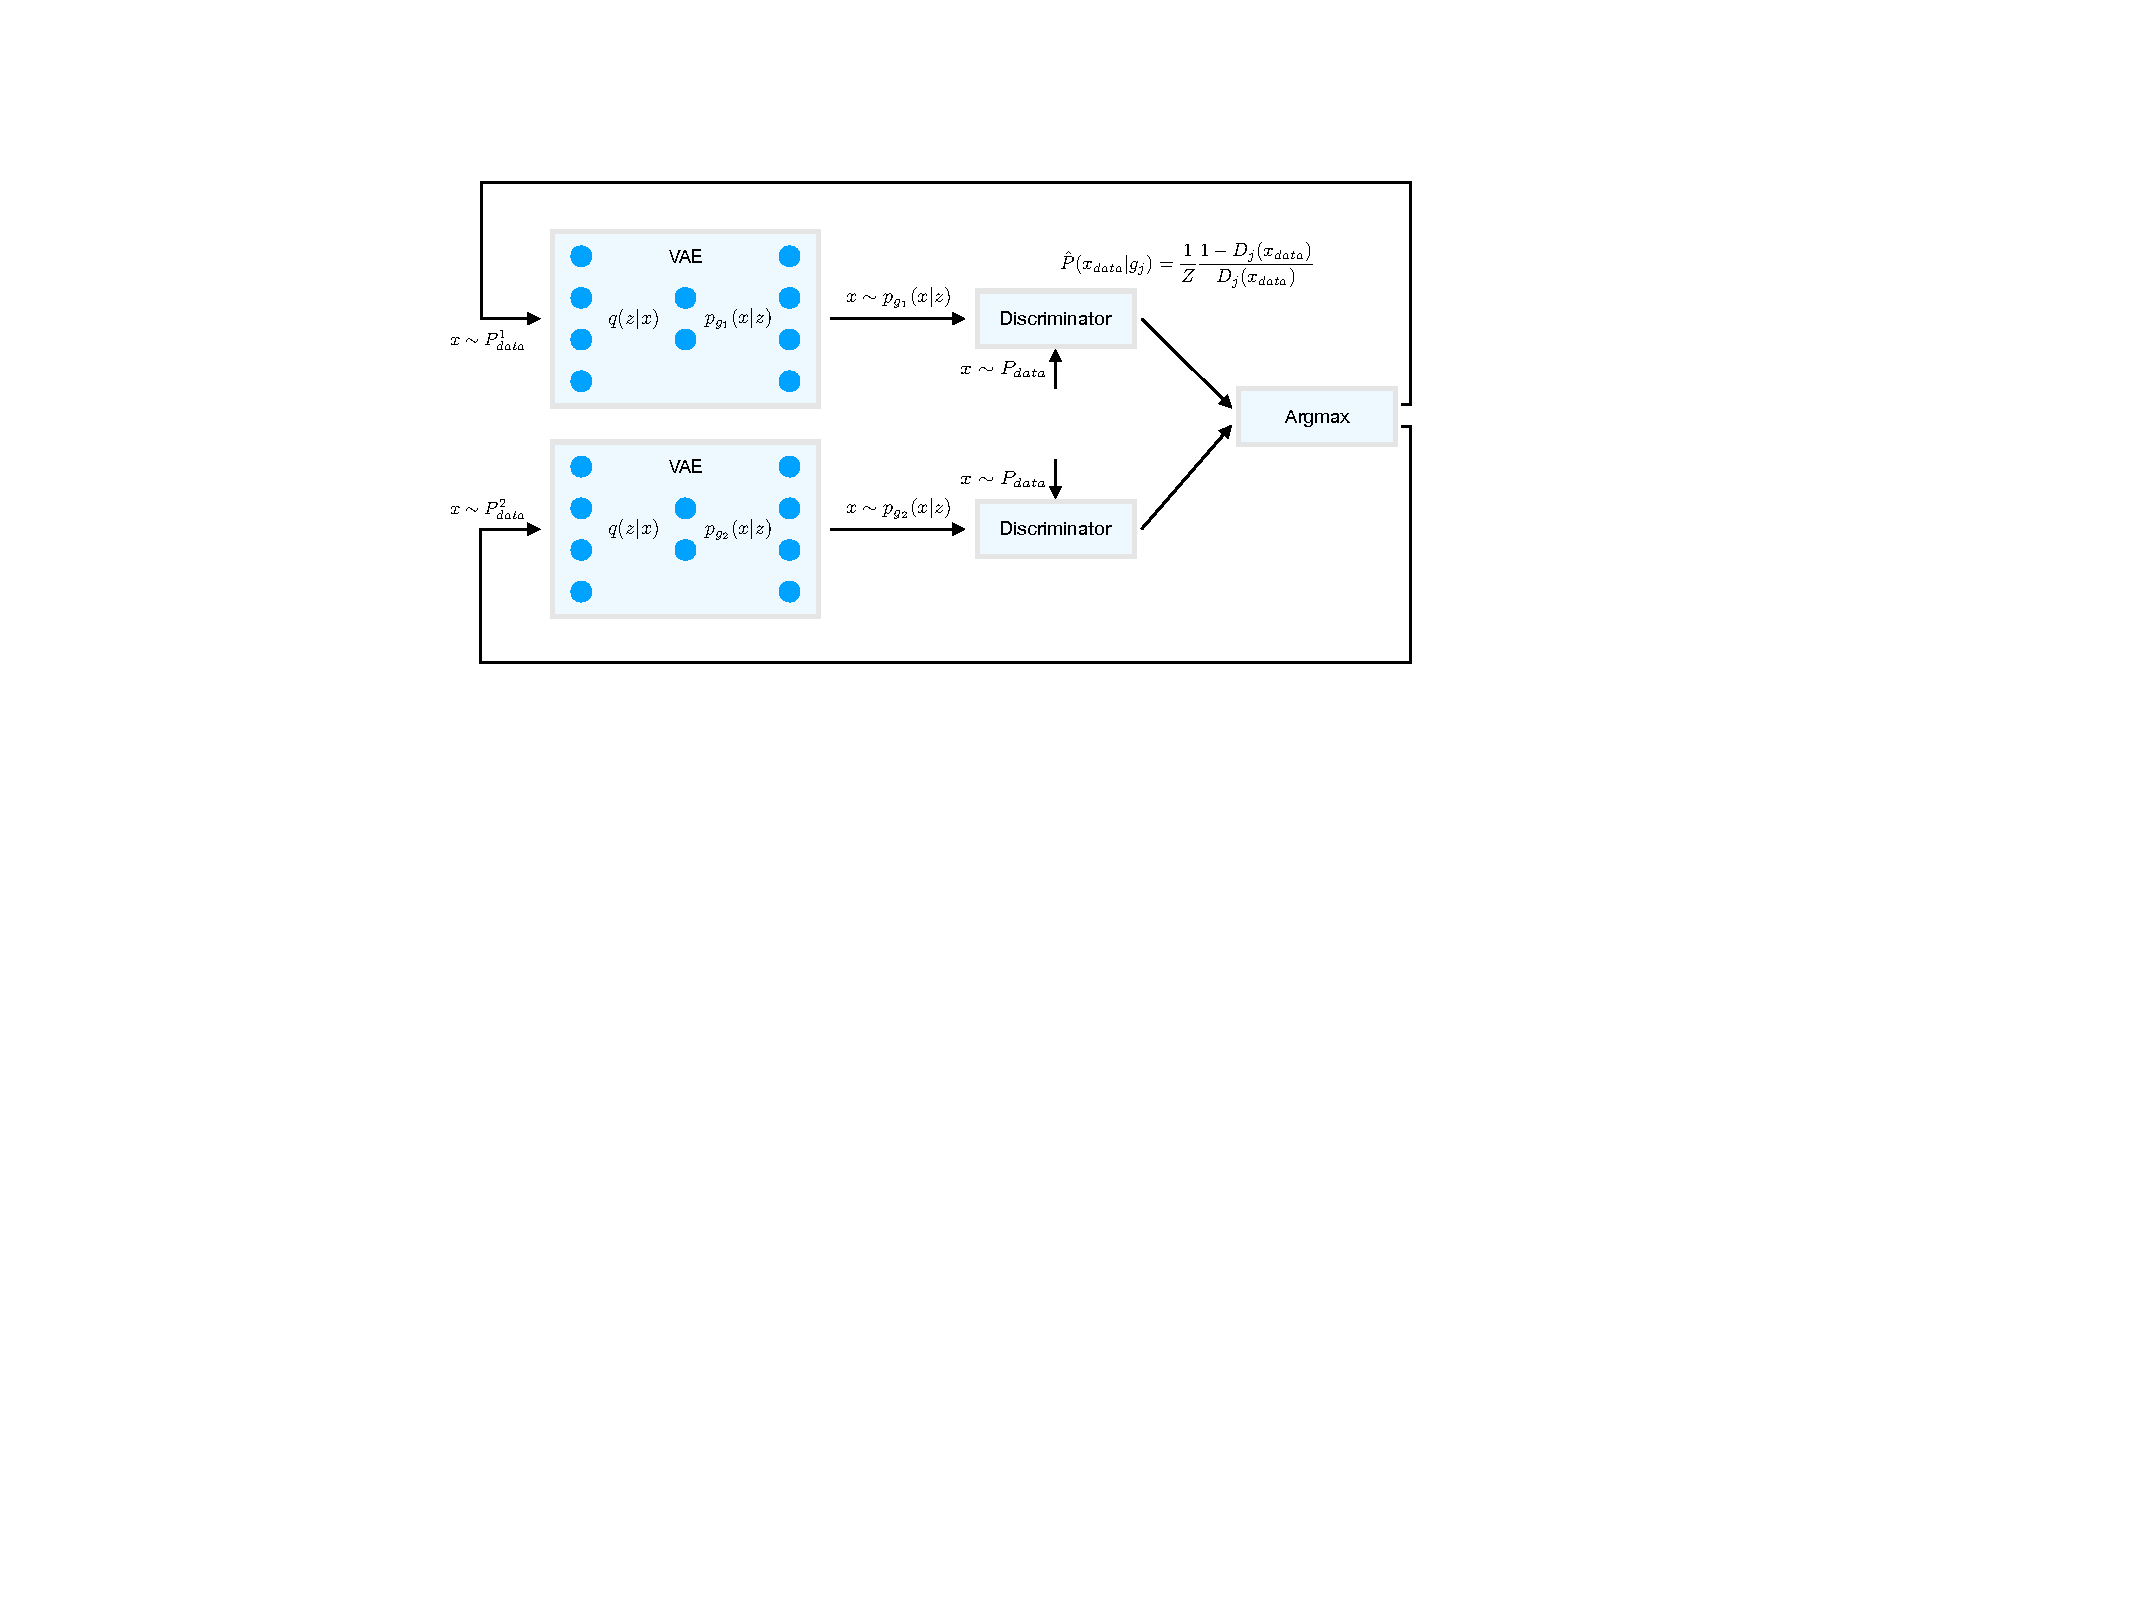
\includegraphics[scale=0.5]{pics/model.pdf}
\end{minipage}\captionof{figure}{Pipeline}\label{fig:model}

 
\section{Convergence}
Let us now fix a particular assignment $c_j = c_j^{(t)}$. As a consequence we write the corresponding portion of the data distribution as $\Pd^{j^{(t)}}$. The optimization problem we need to solve then becomes:
\begin{align*}
\min_{\substack{P_{g_j} \\ j \in [K]}} \alpha_j\sum_j D_f(P_{g_j}| \Pd^{j^{(t)}})
\end{align*}
As every term in the sum is independent from each other, we can minimize them separately, which results in training $K$ generative models approximating $d\Pd^{j^{(t)}}$.

After training each model in parallel, we fix the generators and re-compute the assignment function based on how realistic are the samples produced by each model. Concretely:
 \[
   c_j^{(t+1)}(\bx_i) = \left\{\begin{array}{ll}
        1, & \text{if } j = \argmax_l dP_{g_l}^{(t+1)}(\bx_i) \\
        0, & \text{otherwise }
        \end{array}\right. 
  \]
  where $dP_{g_l}^{(t+1)}(\bx_i)$ can be approximated by training a classifier between $dP_{g_j}$ and $d\Pd$ as in Equation~\eqref{eq:classifier} . 
  \begin{theorem}
  This choice of $c_j$ minimizes the empirical estimate of the loss in Equation~\eqref{eq:objective} for a fixed set of generators with support contained in $\sfX$ and a fixed perfect discriminator. 
  \begin{proof}
  We want to minimize:
  \begin{align*}
 \sum_j \alpha_j D_f\left(P_{g_j}^{(t)}\|c_j(\Pd)\right)
  \end{align*}
  which we rewrite using the properties of $c$ and definition of $\alpha_j$ as: 
  \begin{align}
   \sum_j \alpha_j D_f\left(P_{g_j}^{(t)}\|c_j(\Pd)\right) =  \sum_j  \int_{\sfX} d\Pd c_j \left(f\left(\frac{dP_{g_j}^{(t)}}{d\Pd}\right)\right)
  \end{align}
We can push the finite sum inside the integral, therefore, for each $x\in\sfX$ we need to find the $j$ that maximize $f\left(\frac{dP_{g_j}^{(t)}}{d\Pd}\right)$. 
 Now we turn to the empirical estimate of the loss and exchange the sums: 
 \begin{align*}
 \sum_{x\in\bX}  \sum_j \frac{1}{N} c_j \left(f\left({dP_{g_j}^{(t)}(x)N}\right)\right)
 \end{align*}
 Therefore, due to the definition of $c_j$, we need to find for every $x$ the index $j$ that maximize $dP_{g_j}^{(t)}(x)$
  \end{proof}
  \end{theorem}  
\begin{corollary}\label{cor:decrease}
Since each step at least decreases the objective it holds that:
\begin{align*}
F(c^{(t)},P^{(t)}_{g}) \geq F(c^{(t)},P_{g}^{(t+1)}) \geq F(c^{(t+1)},P_{g}^{(t+1)}) \geq 0 
\end{align*}
where $F$ is the empirical loss.
Therefore, the algorithm converges.
\end{corollary}  
 \begin{theorem}
 The described algorithm converges in finitely many iterations if the non convex optimization problem
 \begin{align*}
 \min_{P_{g_j}}F(c_j^{(t)},P_{g_j})
 \end{align*} 
 has finitely many local minima with different function value.
 \begin{proof}
There are only $N^K$ possible assignments for the points in the training set. For each possible assignment there are finitely many solutions of $\min_{P_{g_j}}F(c_j^{(t)},P_{g_j})$ but they all have to decrease the objective.
We need to show that the same pair of assignment function and generator cannot happen twice unless the algorithm has converged. In other words, the sequence of $c^{(t)}$ and $P^{(t)}_{g}$ does not contain loops.
Assume $c_j^{(t+k)} = c_j^{(t)}$ and $P_{g}^{(t+k)} = P_{g}^{(t)}$ with $k>1$ but the algorithm did not converge, therefore there is at least a single $k' \in [1,k-1]$ s.t $F(c_j^{(t+k')}, P_{g}^{(t+k')})<F(c_j^{(t+k'-1)}, P_{g}^{(t+k'-1)})$. This trivially contradicts Corollary~\ref{cor:decrease} as $F(c_j^{(t+k)}, P_{g}^{(t+k)})=F(c_j^{(t)}, P_{g}^{(t)})$.
 \end{proof}
 \end{theorem}
  
Note that convergence in finitely many iteration is guaranteed only if the minimization wrt the generators has only finitely many local minima with different function value.
\section{kVAEs}
We now particularize the framework using VAEs. One of the reasons to prefer VAEs instead of GANs in this framework is that the adversarial training, with a target that constantly changes, is very unstable and if a single GAN fails the whole model fails. Another reason to use VAE is to better understand their blurriness. Indeed, one of the explanations for the sharpness of the images generated by GANs is that they tend to collapse on a small number of modes from which the model is able to sample points which looks very realistic. In practice, it can happen that a generative model is not expressive enough to perfectly model a complex distribution. In such a case GANs will focus on a part of the data distribution and ignore the parts which are too difficult to approximate. VAEs instead try to cover the whole data distribution as a consequence of minimizing the KL divergence.
Indeed, the vae objective is:
\begin{align}
\cL &=
\bbE_{\bx\sim\Pd} \left[\bbE_{\bz\sim Q} \log P_g(\bx|\bz) - D^{KL}(Q(\bz|\bx)\| P(\bz))\right]
\end{align}
and after the reparametrization trick with gaussian encoder: 
\begin{align}
\cL &=\bbE_{\bx\sim\Pd} \left[\bbE_{\epsilon\sim \cN(0,1)} \log P_g(\bx|\bz = \mu(\bx) + \Sigma^{\frac{1}{2}}(\bx)\epsilon)\right.\nonumber \\ 
&- \left. D^{KL}(Q(\bz|\bx)\| P(\bz))\right],
\end{align}
see~\cite{kingma2013auto}.
The aim is to maximize this loss wrt the parameters of the encoders and the generator (decoder). If $P_g(\bx|\bz) = 0$ for a point in the data distribution the VAE incurs in infinite loss.
Therefore, VAEs when used as generative models produce \textit{bridges} between the modes as one can see in Figure~\ref{pic:blurry}. While we do not claim that the \textit{only} reason for blurriness are samples out of the support of the data distribution, we argue that it is unlikely that these samples are visually realistic. Furthermore, if one wants to claim that the model approximate the data distribution well, there should be an incentive for the support to be as close as possible to $\sfX$. In particular, if $\sfX$ is disjoint, $\Pm$ should also have disjoint support.

In Figure~\ref{pic:blurry} is depicted a VAE trained for 100 epochs whose capacity is the same of the one used in our experimental evaluation.
\begin{minipage}{0.5\textwidth}
\center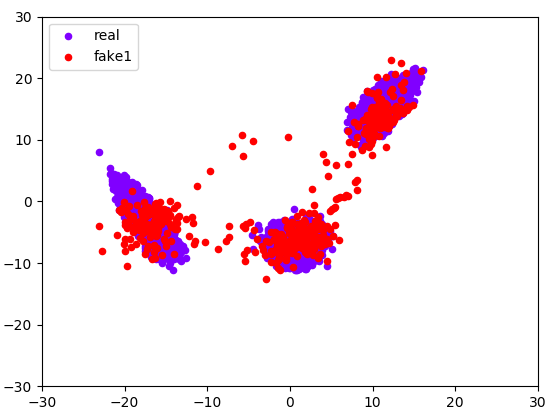
\includegraphics[scale=0.3]{pics/gmm_blurry.png}
\end{minipage}\captionof{figure}{VAE producing samples outside the data distribution}\label{pic:blurry}

\section{Clustering Interpretation}
The general approach we introduced is inspired by clustering literature \cite{aggarwal2013data}. In this section we revisit classical clustering notions under the lights of our framework.  In the generative interpretation of clustering, one assumes that the data was generated from each centroid by sampling gaussian noise vector. We can say that $x = c + \epsilon$ where $c$ is the centroid. This formulation naturally yields an euclidean cost for the cluster assignment when decoupling the data between the different centroids. Unfortunately, the euclidean distance is known not to be a good metric in a non-euclidean space such as the pixel space. Our goal is to find a clustering of the data across the generating mechanism in a setting in which the metric of the space is not known. We now show how to recover the k-means clustering from our framework.
Assume that the data is generated by a mixture of gaussians. We can lower bound the log likelihood of the data using a variational bound:
\begin{align*}
\log(P(X)) \geq \sum_n \sum_{z_i} q_n(z_i) \log\left( \frac{P(x_n,z_i)}{q_n(z_i)}\right)
\end{align*}
 where $q$ is the variational distribution. One can then simply rewrite $P(x_n,z_i) = P(x_n|z_i)p(z_i)$. Then, for a gaussian mixture model one parametrize $P(x_n|z_i)$ with a gaussian distribution. If the gaussian is isometric, when the covariance vanishes one obtains that $q_n(z_i)$, the variational approximation of the posterior, degenerates to a hard assignment. Instead of approximating the generative model with a gaussian distribution, we parametrize $P(x_n|z_i)$ with an implicit generative model from which is easy to sample. If $P_{g_i}$ is the decoder of a variational autoencoder, we can obtain the k-means algorithm by assuming that the mean of the encoder is constant and independent of $x$. The latent space of the variational autoencoder has the same dimensionality of the input but is independent from the input. Then we have a gaussian decoder with no covariance. The result of this procedure is that when training the autencoder with the reparametrization trick one has to minimize:
 \begin{align*}
 \bbE_{x\sim c_j(\Pd)} - \log P_g(x|z = \mu) =  \frac{1}{2}\|x - \mu \|^2
 \end{align*}
 The only parameters to optimize are the biases of the encoder, i.e. $\mu$ for the assigned points. Then, using EM, we compute the update for the (degenerate) variational distribution:
 \begin{align*}
 q_n(z_i = 1) = \lim_{\sigma\rightarrow 0} \frac{\alpha e^{-\|x_n-\mu_i\|/2\sigma}}{\sum_j\alpha_je^{-\|x_n-\mu_j\|/2\sigma}}
 \end{align*}
And recalling that $\log P_{g_i} = - \| x_n -\mu_i \|^2/2$ we notice that our assignment update corresponds in this case to maximizing the posterior assignment as typically done in k-means. Instead of using the autencoder loss, we estimate $P_{g_j}$ using a discriminator to account for the fact that we might not have a clear notion of distance. 
When testing the model (i.e. generating samples from the centroids) we simply input values from a normal distribution to the gaussian decoder and $x = \mu + \epsilon$.

\section{Related Work}

\section{Experimental Proof of Concept}
In this section we evaluate the proposed framework. We want to test if the model can successfully learn disentangled generative mechanisms for the data.
\FL{add more on the goal of the experiments}

\subsection{Synthetic Data}
We generate synthetic data in 2 dimension by first sampling 64000 points from a gaussian distribution and then we skew the second dimension $x_2$ with the non linear transformation $x_2 = x_2 +  0.04 * x_1^2 - 100 *  0.04$. This ensures that each mode is sufficiently complex so that the VAEs can not perfectly learn the data distribution by encoding each mode on a different dimension of the latent space. We use a small and standard architecture for the VAE: a neural network with two hidden layers with 500 units each as both decoder, encoder and discriminator.
We use a 5 dimensional latent space and assume a gaussian encoder. At each iteration, we train each VAE for 10 epochs on a split of the dataset (VAEs are pretrained uniformly on the dataset) and the classifier is trained for 2 epochs for the first two experiments. We use adam with step size 0.005, $\beta = 0.5$ batch size 32 and batch norm with decay $0.9$. We perform 3 different experiments, 3 modes (and 3 VAEs), 5 modes (and 5 VAEs) in which one mode is actually composed of two separate modes which are very close and 9 modes (with 9 VAEs). We run the algorithm for 100 iterations. We note that in the first two experiments each model perfectly cover a single mode, even in the case in which there is a mode which is distributed differently. In the last experiments, each mode contains significantly fewer points than the previous ones. In this case, we first train each VAE for 1000 epochs. We note that even after training for so long the models perform very poorly, because the data is far too complex for such simple models. Then, we run our algorithm on the pretrained models and each model is reatrained for 10 epochs on the split given by the classifier. Surprisingly, after only 10 iterations of the algorithm the model splits covering only limited parts of the data distribution. We still observe that some model still try to approximate multiple modes yielding samples outside the support of the data distribution. Note that the only incentive for the model to split is the competitive procedure which we use to assign the data to each VAE. \FL{comment the log likelihood}
\begin{table*}
\begin{center}
\begin{tabular}{ l | c | c | c | c  }
  experiment & kVAEs train/test & bag train/test & VAE-50 train/test & VAE-150 train/test\\
  \hline
  gmm 3 modes & \textbf{-3.36} / \textbf{-3.47} & TODO/TODO &-6.21 / 6.08 & -5.79 / -5.92\\			
  gmm 5 modes & \textbf{-1.25} / \textbf{-1.29} & TODO/TODO & -5.38 / -5.54 & -5.39 / -5.66\\
  gmm 9 modes & \textbf{-0.97} / \textbf{ -0.99} & TODO/ TODO & -4.08 / -4.04 & -3.95 / -4.23\\  
\end{tabular}
\end{center}
\end{table*}

\begin{minipage}{0.5\textwidth}
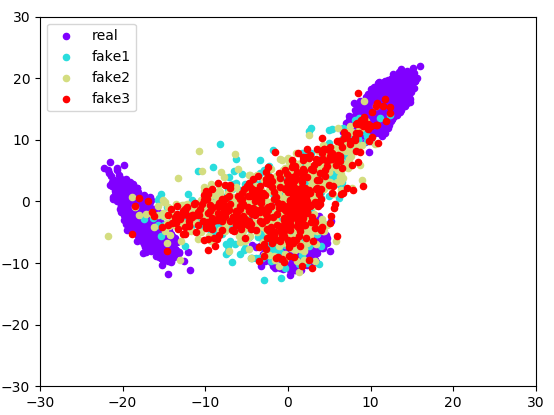
\includegraphics[scale=0.21]{pics/gmm_3_0.png}
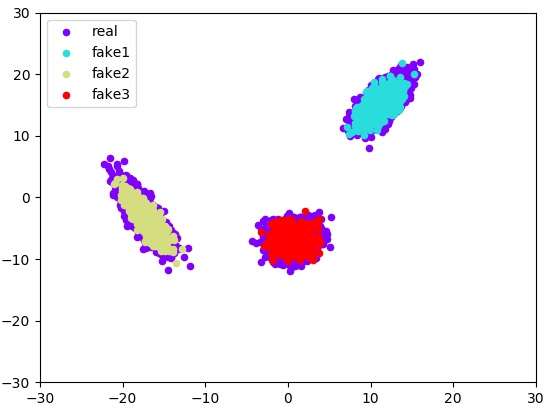
\includegraphics[scale=0.21]{pics/gmm_3_100.png}
\end{minipage}\captionof{figure}{Synthetic data experiment, 3 modes, uniform training and after 100 iterations of the algorithm.}

\begin{minipage}{0.5\textwidth}
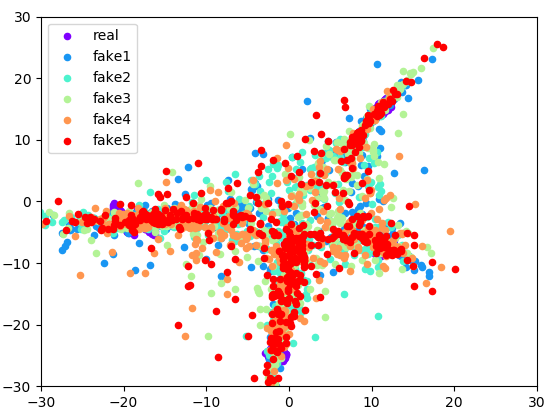
\includegraphics[scale=0.21]{pics/gmm_5_0.png}
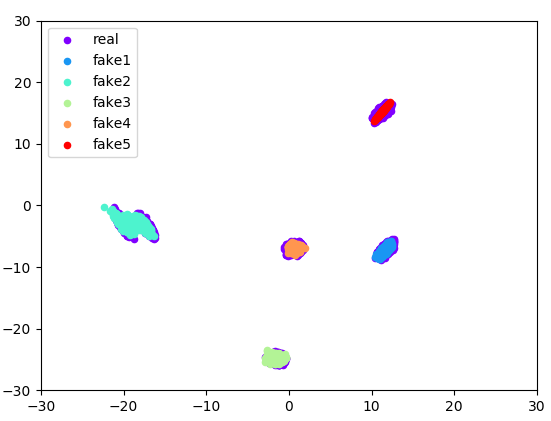
\includegraphics[scale=0.21]{pics/gmm_5_100.png}
\end{minipage}\captionof{figure}{Synthetic data experiment, 5 modes, uniform training and after 100 iterations of the algorithm.}
\begin{figure*}
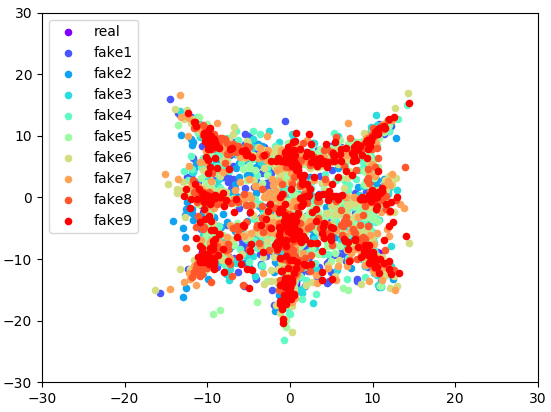
\includegraphics[scale=0.31]{pics/gmm_9_0.png}
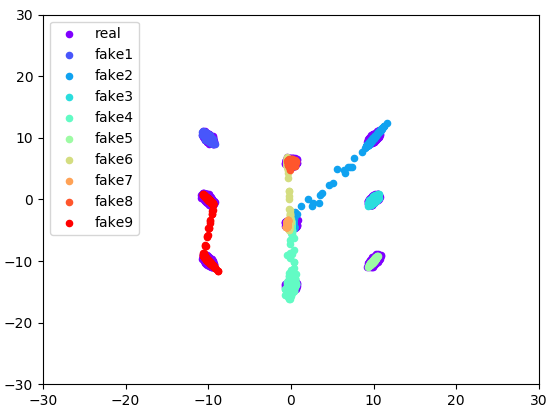
\includegraphics[scale=0.31]{pics/gmm_9_10.png}
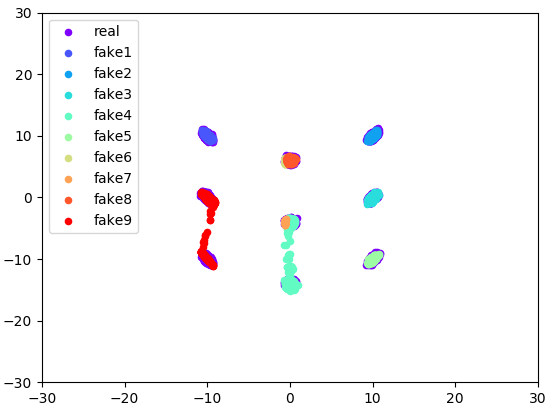
\includegraphics[scale=0.31]{pics/gmm_9_100.png}
\caption{Synthetic data experiment, 9 modes, uniform training and after 10 and 100 iterations of the algorithm.}
\end{figure*}
\subsection{MNIST}
For the experiment on MNIST we do not know the number of modes. Therefore we arbitrarily fix 15 models. We decided to use more than 10 models as, following the insights from~\cite{Tolstikhin:2017wo}, we were targeting stylistic difference between digits. Indeed, different modes might not be coincides with different classes. 
We again use a small and simple architecture, with relu activation functions. The encoder has 4 convolutional layers with 8-16-32-64 filters with 4 dimensions each. The decoder has 4 deconvolutional layers, with  the same number of filters as the decoder. We use batch normalization with epsilon $1e-5$ and decay $0.9$. Each VAE has latent space dimension of $8$ and we fix the learning rate of Adam for all networks to $0.005$. 
The discriminator is has 3 convolutional layers and a linear layer with number of filters 64-128-256. As opposed to the synthetic data example, we do not reinitialize the classifier each iteration. Instead, we train it for a single batch every iteration. The reason is that we found the classifier output to be too sensitive to the initialization if it is not trained long enough. On the other hand, training a full discriminator every iteration was too expensive and if trained too much it would learn to distinguish fake example by just looking at specific blurriness patterns. On the other hand, the data produced by the VAE in the synthetic experiments was indistinguishable from the real data, so training a classifier from scratch was feasible and gave best results.
In Figure~\ref{fig:mnist_assign} we show the number of training samples assigned to each model divided by digit and in Figure~\ref{fig:mnist_comp} samples from each decoder. We highlight that the different VAEs did separate the data and specialized on different parts of the data distribution. We notice that similar digits tends to be grouped together (for example 3 and 8, 6 and 4) as well as similar styles (tilted, thin, large, round, bold and combinations thereof). Since it is not clear what the modes are supposed to be, we also show samples from the whole mixture and notice that there is a large variety of different styles.
\FL{Comment the log likelihood}
\begin{minipage}{0.5\textwidth}
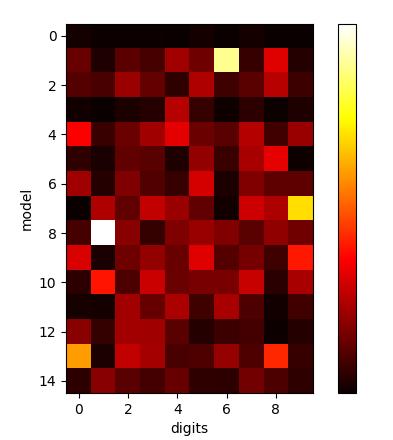
\includegraphics[scale=0.3]{pics/mnist_assign_0.png}
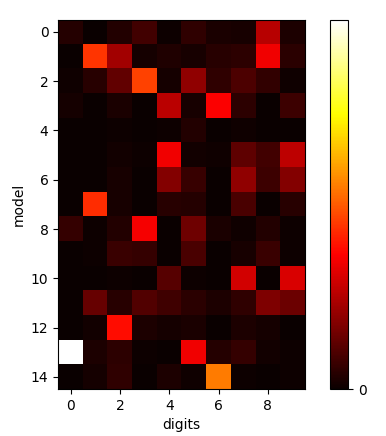
\includegraphics[scale=0.3]{pics/mnist_assign_99.png}
\end{minipage}\captionof{figure}{MNIST assignments: how many points with the same label are assigned to each model}\label{fig:mnist_assign}

\begin{figure*}
\center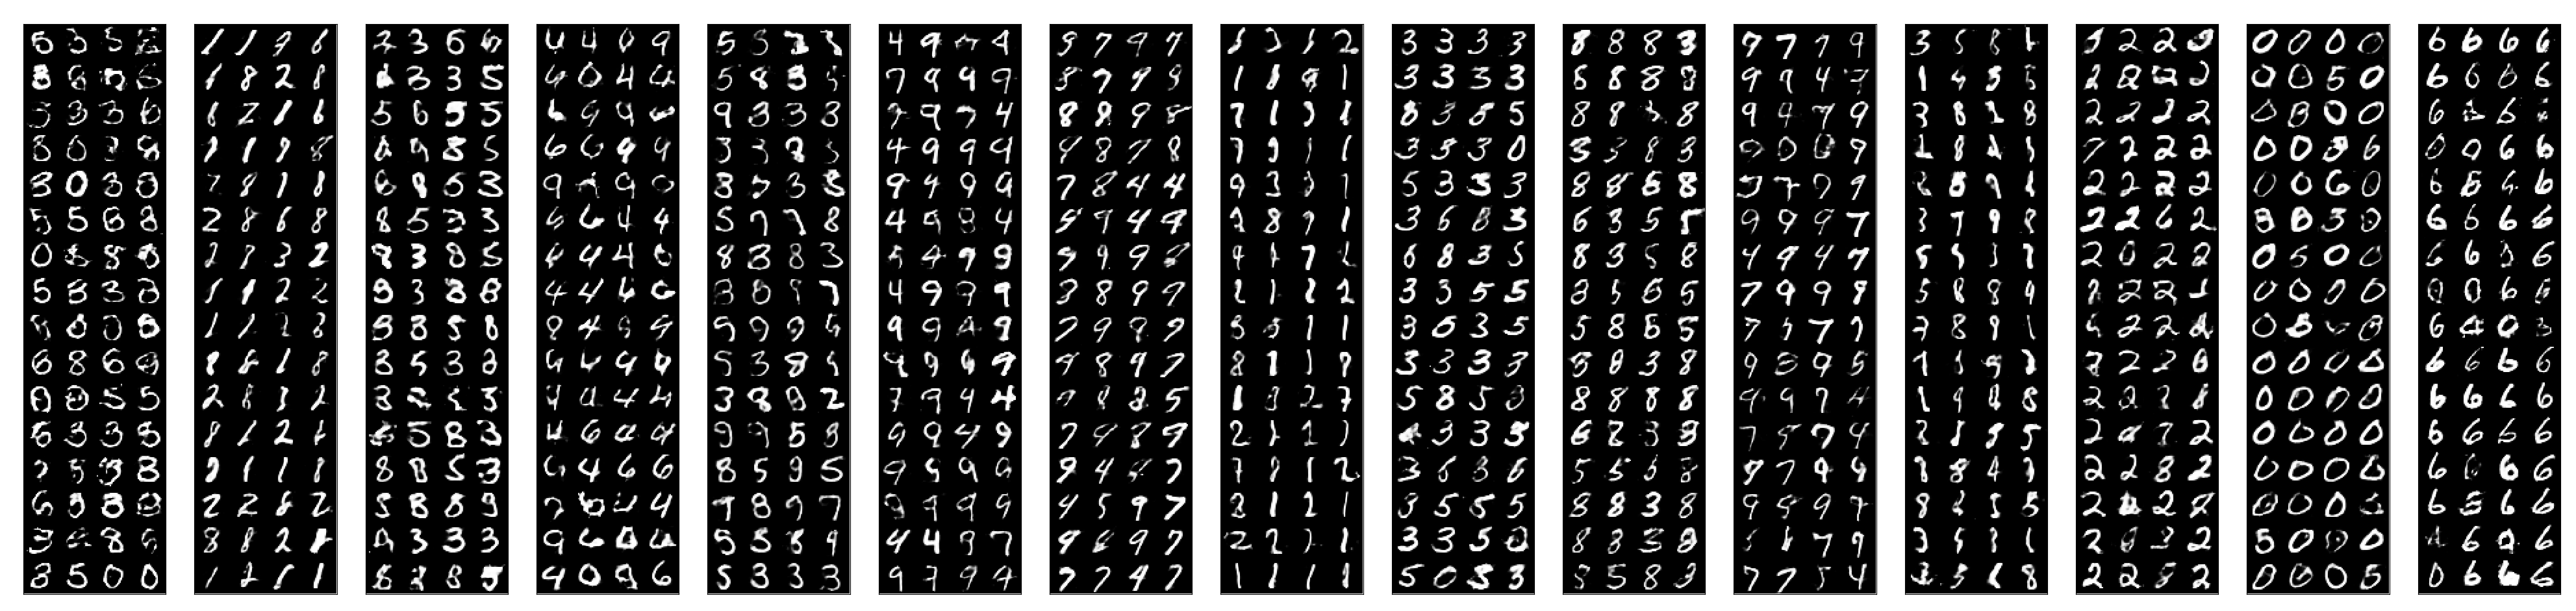
\includegraphics[scale=0.12]{pics/mnist_comp_99.png}
\caption{MNIST: samples separated per model}\label{fig:mnist_comp}
\end{figure*}
\begin{figure*}
\center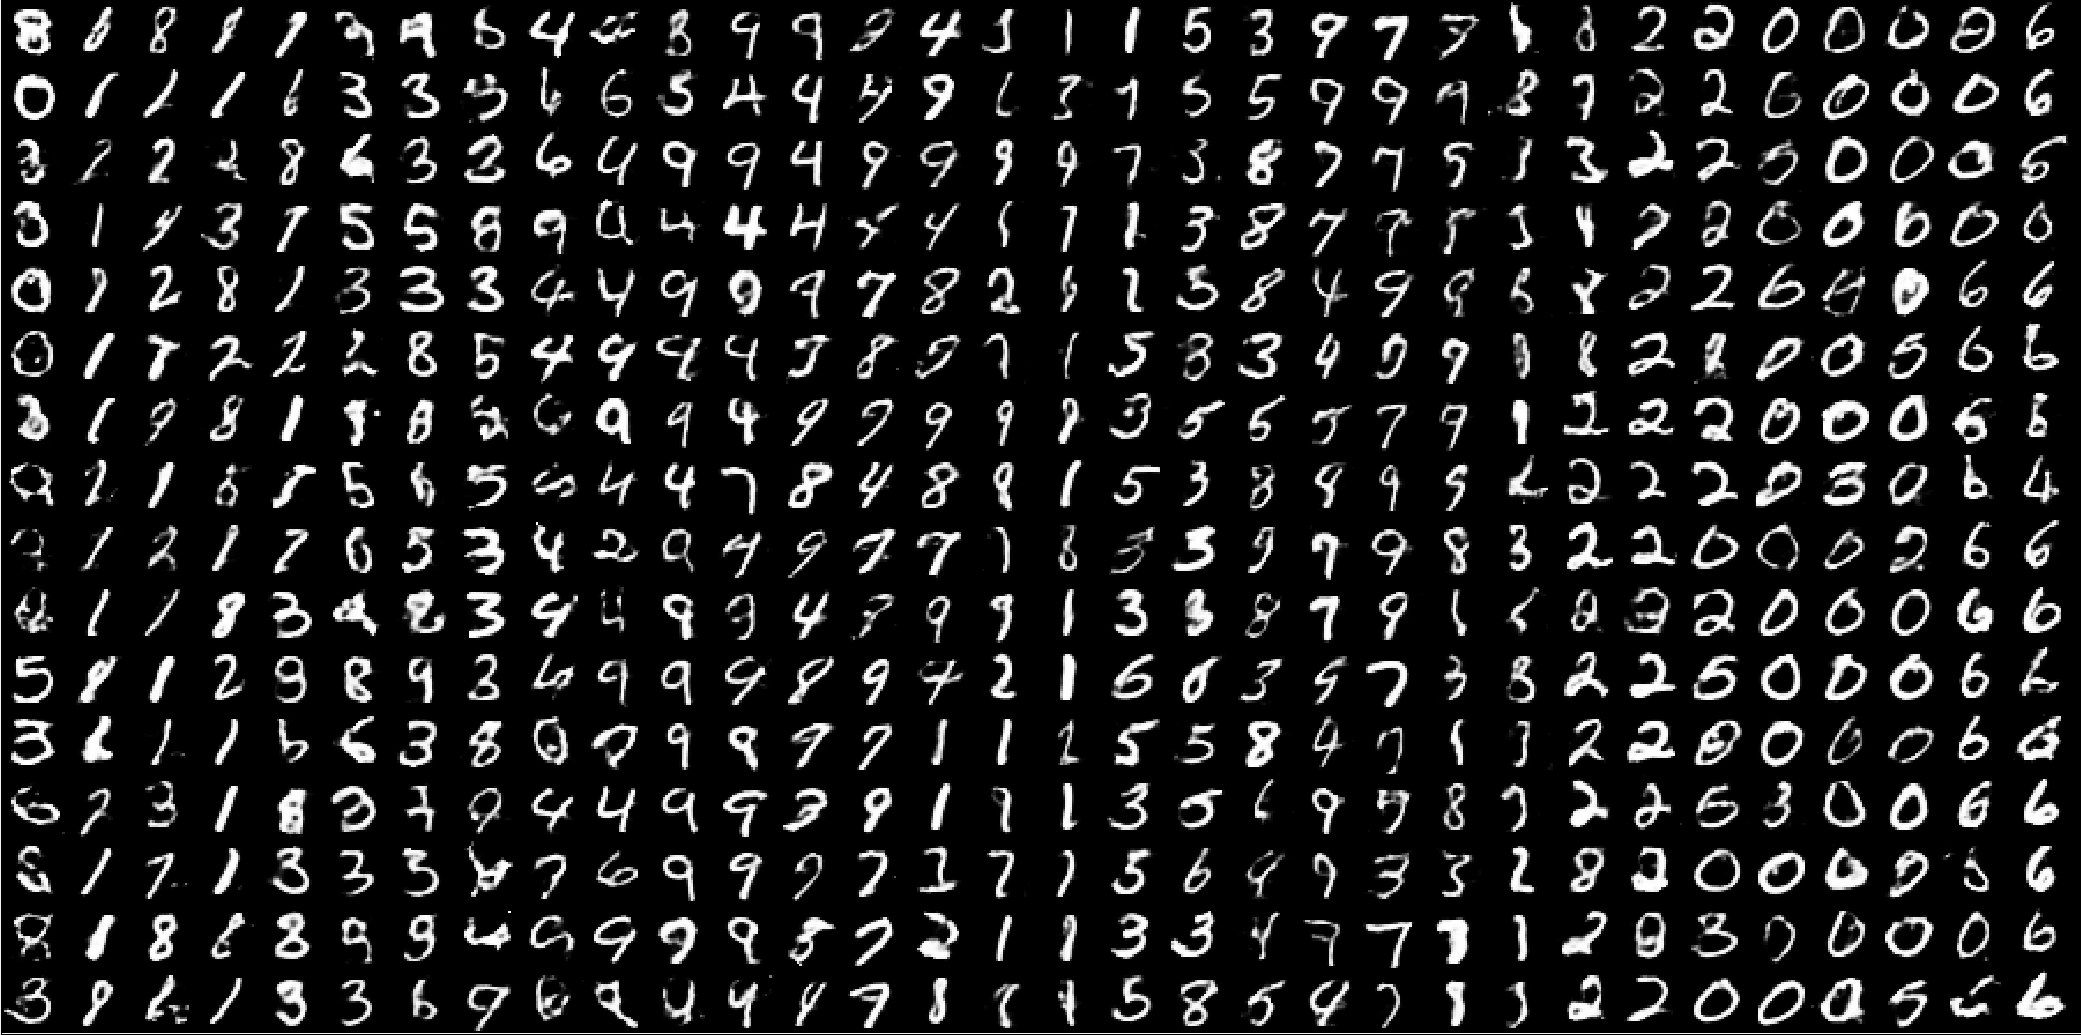
\includegraphics[scale=0.2]{pics/mnist_mixture_99.png}
\caption{MNIST: samples from the mixture}\label{fig:mnist_mix}
\end{figure*}

\begin{table*}
\begin{center}
\begin{tabular}{ l | c | c | c | c | c | c }
  kVAEs train/test & bag train/test & VAE-64 train/test &VAE-512 train/test & VAE-1024 train/test\\
  \hline
 TODO / TODO &TODO / TODO & - 3.12e+03/ - 3.28e+03 &-1.63e+04 / -5.32e+04	& -1.64e+04/ -5.34e+04 	
\end{tabular}
\end{center}
\end{table*}
\paragraph{Selecting K}
Selecting the number of models is a question which does not have a trivial answer. It is not reasonable to assume that one can fix a large $K$ and the extra models will just be defeated in the competitive procedure. Indeed, as in k-means clustering, if $K$ is too large we would simply fit more models which in turns will yield to an unstable clustering. On the other hand, the extra models will have very few points assigned, thus the mixture will contain only a few of their samples. For these experiments, we fixed a priori the number of VAEs without tuning it as we wanted to demonstrate that the algorithm behaves as expected. Solutions for finding $K$ involving stability of the clustering are unfortunately unfeasible (as running the algorithm several times is time consuming). Finding an efficient technique to estimate $K$ while the algorithm run is an interesting future direction.
\clearpage
\newpage
\bibliography{bibliography}
\bibliographystyle{icml2018}


%%%%%%%%%%%%%%%%%%%%%%%%%%%%%%%%%%%%%%%%%%%%%%%%%%%%%%%%%%%%%%%%%%%%%%%%%%%%%%%
%%%%%%%%%%%%%%%%%%%%%%%%%%%%%%%%%%%%%%%%%%%%%%%%%%%%%%%%%%%%%%%%%%%%%%%%%%%%%%%
% DELETE THIS PART. DO NOT PLACE CONTENT AFTER THE REFERENCES!
%%%%%%%%%%%%%%%%%%%%%%%%%%%%%%%%%%%%%%%%%%%%%%%%%%%%%%%%%%%%%%%%%%%%%%%%%%%%%%%
%%%%%%%%%%%%%%%%%%%%%%%%%%%%%%%%%%%%%%%%%%%%%%%%%%%%%%%%%%%%%%%%%%%%%%%%%%%%%%%

\appendix

%%%%%%%%%%%%%%%%%%%%%%%%%%%%%%%%%%%%%%%%%%%%%%%%%%%%%%%%%%%%%%%%%%%%%%%%%%%%%%%
%%%%%%%%%%%%%%%%%%%%%%%%%%%%%%%%%%%%%%%%%%%%%%%%%%%%%%%%%%%%%%%%%%%%%%%%%%%%%%%


\end{document}


% This document was modified from the file originally made available by
% Pat Langley and Andrea Danyluk for ICML-2K. This version was created
% by Iain Murray in 2018. It was modified from a version from Dan Roy in
% 2017, which was based on a version from Lise Getoor and Tobias
% Scheffer, which was slightly modified from the 2010 version by
% Thorsten Joachims & Johannes Fuernkranz, slightly modified from the
% 2009 version by Kiri Wagstaff and Sam Roweis's 2008 version, which is
% slightly modified from Prasad Tadepalli's 2007 version which is a
% lightly changed version of the previous year's version by Andrew
% Moore, which was in turn edited from those of Kristian Kersting and
% Codrina Lauth. Alex Smola contributed to the algorithmic style files.
